\appendix
\chapter{Risk Analysis}

\begin{figure}[H]
\centering
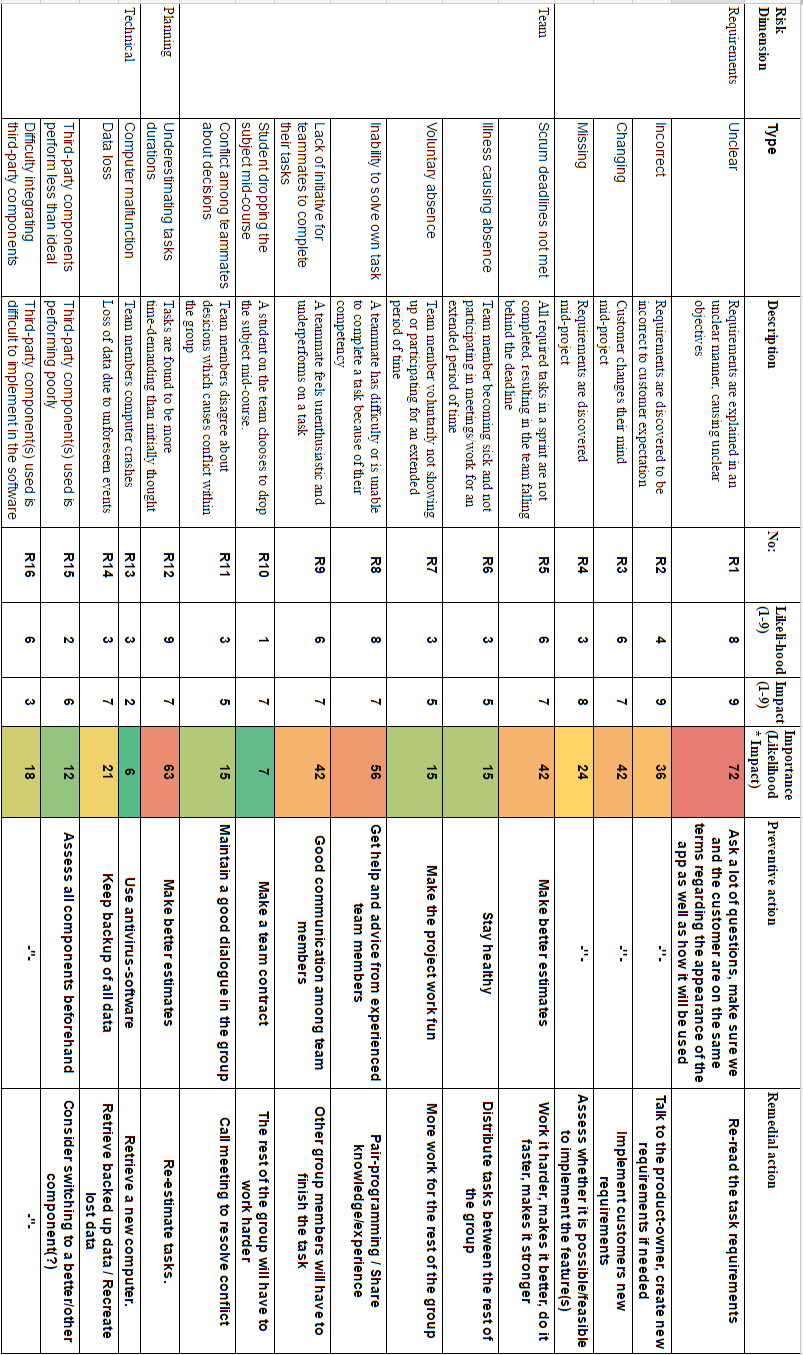
\includegraphics[scale=0.50]{Figures/riskMatrixBLA.png}
\caption{Risk Analysis}
\label{fig:RiskFull}
\end{figure}

\chapter{Sprints}
\section{Sprint 1}\label{sprint1}

\begin{figure}[H]
\centering
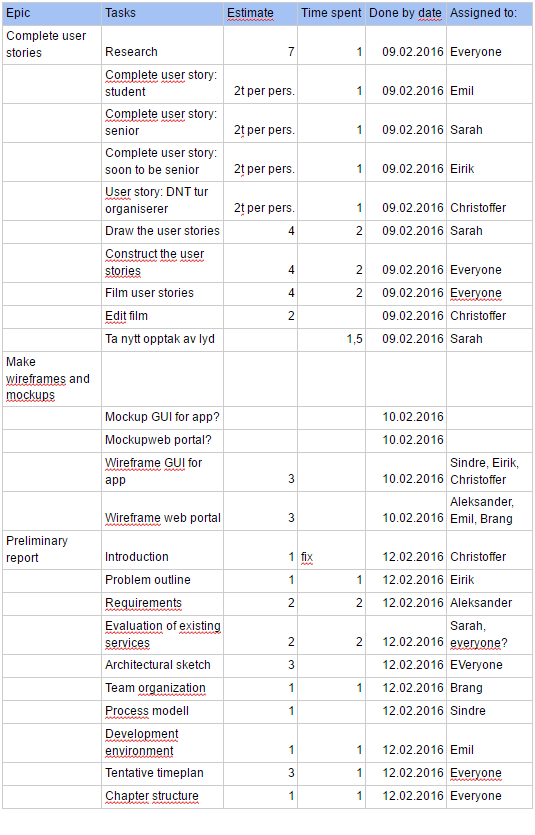
\includegraphics[width = 0.75\textwidth]{Figures/sprints/sprint1}
\caption{Sprint 1}
    \label{fig:SP1}
    \end{figure}

\section{Sprint 2}\label{sprint2}

\begin{figure}[H]
\centering
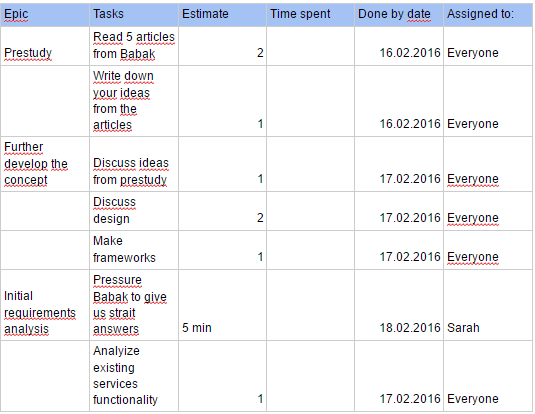
\includegraphics[width = 0.75\textwidth]{Figures/sprints/sprint2}
\caption{Sprint 2}
    \label{fig:SP2}
    \end{figure}

\section{Sprint 3}\label{sprint3}

\begin{figure}[H]
\centering
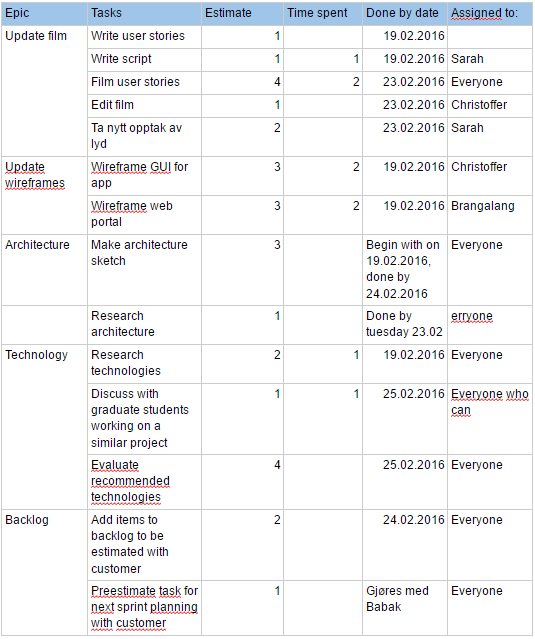
\includegraphics[width = 0.75\textwidth]{Figures/sprints/sprint3}
\caption{Sprint 3}
    \label{fig:SP3}
    \end{figure}

\section{Sprint 4}\label{sprint4}

\begin{figure}[H]
\centering
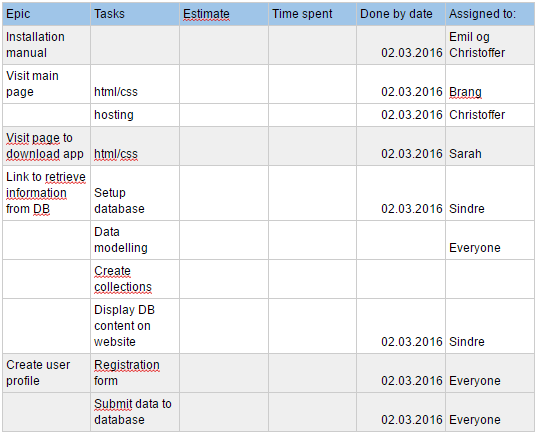
\includegraphics[width = 0.75\textwidth]{Figures/sprints/sprint4}
\caption{Sprint 4}
    \label{fig:SP4}
    \end{figure}

\section{Sprint 5}\label{sprint5}

\begin{figure}[H]
\centering
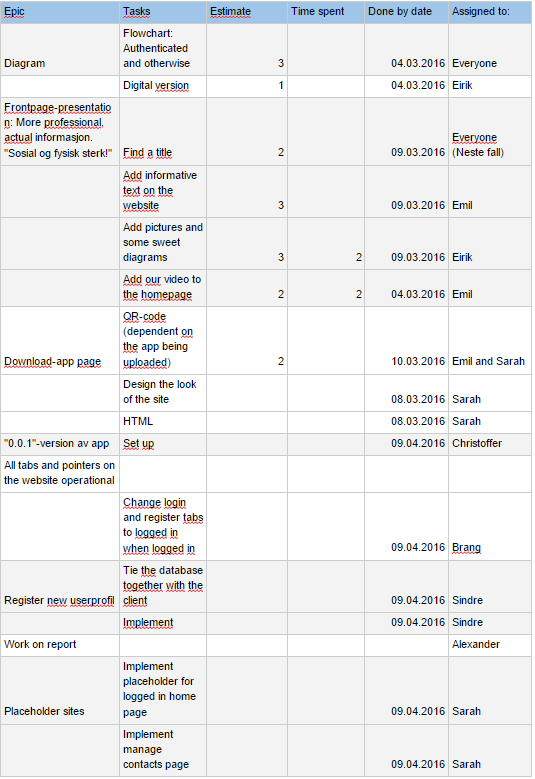
\includegraphics[width = 0.75\textwidth]{Figures/sprints/sprint5}
\caption{Sprint 5}
    \label{fig:SP5}
    \end{figure}

\section{Sprint 6}\label{sprint6}

\begin{figure}[H]
\centering
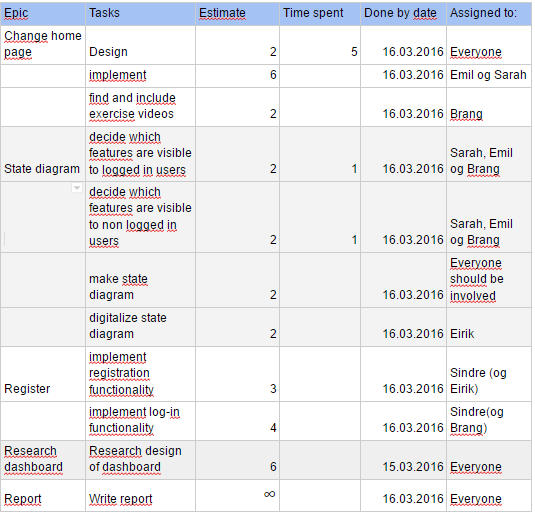
\includegraphics[width = 0.75\textwidth]{Figures/sprints/sprint6}
\caption{Sprint 6}
    \label{fig:SP6}
    \end{figure}

\section{Sprint 7}\label{sprint7}
The full sprint backlog for this sprint can be found on gitHub at \cite{sprint7}
\section{Sprint 8}\label{sprint8}
The full sprint backlog for this sprint can be found on gitHub at \cite{sprint8}
\section{Sprint 9}\label{sprint9}
The full sprint backlog for this sprint can be found on gitHub at \cite{sprint9}
\section{Sprint 10}\label{sprint10}
The full sprint backlog for this sprint can be found on gitHub at \cite{sprint10}


\chapter{Unit Tests}\label{unitTests}
\begin{table}[H]
\begin{tabular}{ | L{0.25\linewidth} | L{0.75\linewidth} | } 
 \hline \rowcolor{lightgray}
 Unit Test 1 &  \\
 \hline
 Test Item & Register user profile and log in as registered user \\ 
 \hline
 Test functional requirements no: & F1, F2
 \\ 
 \hline
 Approach & Register new user and log in with the provided details. \\ 
  \hline
 Item pass/fail criteria &  If webpage is not accessed, the test fails. If register does not work, the test fails, if login with the provided details from register does not work, the test fails. If users can register and log in with the provided details, the test passes. \\ 
 \hline
 Input &  Username, email and password\\ 
 \hline
 Expected results & Dashboard of the newly registered user \\ 
  \hline
Testing task & 
\vspace{-5mm}
    \begin{enumerate}[noitemsep]
  \item Enter website
  \item Click register
  \item Enter email and password
  \item Click log in and provide the same username, email and password
  \item Check if the user is logged in
   \end{enumerate}\\
 \hline
 Necessary environmental requirement & The website is running \\ 
 \hline
\end{tabular}
\caption{Unit test 1}
\end{table}

\begin{table}[H]
\begin{tabular}{ | L{0.25\linewidth} | L{0.75\linewidth} | } 
 \hline \rowcolor{lightgray}
 Unit Test 2 & \\
 \hline
 Test Item & User can edit their own profile information\\ 
 \hline
 Test functional requirements no: & F3
 \\
 \hline
 Approach & User can edit their profile information\\ 
  \hline
 Item pass/fail criteria &  If user clicks edit profile button, and nothing happens, the test fails. If the edited fields are not updated the test fails. If the user clicks edit, edits the fields and they are updated like expected, the test passes.\\ 
 \hline
 Input &  First name, last name, bio, password and profile picture\\ 
 \hline
 Expected results & Profile is edited successfully \\ 
  \hline
Testing task & 
\vspace{-5mm}
    \begin{enumerate}[noitemsep]
  \item User clicks edit profile
  \item User edits fields of their choice
  \item User clicks save
   \end{enumerate}\\
 \hline
 Necessary environmental requirement & The user is logged in and on the profile page\\ 
 \hline
\end{tabular}
\caption{Unit Test 2}
\end{table}

\begin{table}[H]
\begin{tabular}{ | L{0.25\linewidth} | L{0.75\linewidth} | } 
 \hline \rowcolor{lightgray}
 Unit Test 3 &  \\
 \hline
 Test Item & User can create event \\ 
 \hline
 Test functional requirements no: & F4
 \\
 \hline
 Approach & User clicks "createEvent" and fills in event form. Check if event shows up under "Mine aktiviteter" \\ 
  \hline
 Item pass/fail criteria &  If "createEvent" button is non-responsive, the test fails. If form cannot be filled in, the test fails. If event does not show ip in "Mine aktiviteter", the test fails. If event is displayed under "Mine aktiviteter", the test passes  \\ 
 \hline
 Input &  Any of the following: name, description, date, place, participants, type, difficulty level, public\\ 
 \hline
 Expected results & A newly created event displayed under "Mine aktiviteter" \\ 
  \hline
Testing task &
\vspace{-5mm}
    \begin{enumerate}[noitemsep]
  \item Click "Opprett ny aktivitet"
  \item Fill inn all fields of interest
  \item Submit form
  \item Check if event is displayed under "Mine aktiviteter"
   \end{enumerate}\\
 \hline
 Necessary environmental requirement & Successfully logged in to the user's account \\ 
 \hline
\end{tabular}
\caption{Unit test 3}
\end{table}

\begin{table}[H]
\begin{tabular}{ | L{0.25\linewidth} | L{0.75\linewidth} | } 
 \hline \rowcolor{lightgray}
 Unit Test 4 & \\
 \hline
 Test Item & Registered user can search for events\\ 
 \hline
 Test functional requirements no: & F5
 \\
 \hline
 Approach & Registered user can search for events\\ 
  \hline
 Item pass/fail criteria & If the user searches for an event and nothing happens, the test fails. If the user clicks the searched event and nothing happens, the test fails. If the user searches for an event, clicks the event, and is taken to "mine aktiviteter" displaying the chosen event.\\ 
 \hline
 Input &  The searched event\\ 
 \hline
 Expected results & The searched event is displayed \\ 
  \hline
Testing task & 
\vspace{-5mm}
    \begin{enumerate}[noitemsep]
  \item User searches for the event of their choice
  \item User clicks the searched event
   \end{enumerate}\\
 \hline
 Necessary environmental requirement & The user is logged in\\ 
 \hline
\end{tabular}
\caption{Unit Test 4}
\end{table}

\begin{table}[H]
\begin{tabular}{ | L{0.25\linewidth} | L{0.75\linewidth} | } 
 \hline \rowcolor{lightgray}
 Unit Test 5 & \\
 \hline
 Test Item & Registered user can invite friends to event\\ 
 \hline
 Test functional requirements no: & F6
 \\
 \hline
 Approach & User adds friend to event through dropdown menu\\ 
  \hline
 Item pass/fail criteria & If the user clicks "rediger denne aktiviteten" and nothing happens, the test fails. If the user clicks "klikk her for å legge til deltagere" and nothing happens, the test fails. If the user clicks "ferdig" and nothing happens, the test fails. If the user successfully edits the event and add users to the event, the test passes.\\ 
 \hline
 Input &  Searching and adding users\\ 
 \hline
 Expected results & New event with the selected users added to the participant list \\ 
  \hline
Testing task &
\vspace{-5mm}
    \begin{enumerate}[noitemsep]
  \item User clicks "rediger denne aktiviteten" which brings up the modal for editing the event
  \item User clicks "klikk her for å legge til deltagere" and types in the user it wants add and selects it
  \item User clicks "ferdig"
   \end{enumerate}\\
 \hline
 Necessary environmental requirement & The user is logged in and is in "mine aktivteter" and has clicked the event of their choice\\ 
 \hline
\end{tabular}
\caption{Unit Test 5}
\end{table}

\begin{table}[H]
\begin{tabular}{ | L{0.25\linewidth} | L{0.75\linewidth} | } 
 \hline \rowcolor{lightgray}
 Unit Test 6 &  \\
 \hline
 Test Item & Registered user can join other users events\\ 
 \hline
 Test functional requirements no: & F7
 \\ 
 \hline
 Approach & User receives invitation to event, click on it and can choose between "Accept" and "Decline" \\ 
  \hline
 Item pass/fail criteria &  If user cannot see any buttons for "Accept" and "Decline", the test has failed. If the user accepts of declines the invitation, but their status is not updated in eventDetails, the test fails. If the user's status is updated, the test passes  \\ 
 \hline
 Input &  Click on "Accept"/"Decline"\\ 
 \hline
 Expected results & Status updated in event details view \\ 
  \hline
Testing task & 
\vspace{-5mm}
    \begin{enumerate}[noitemsep]
  \item Click on the event invitation
  \item Click on "Accept" or "Decline"
  \item Check if status is updated in event details view.
   \end{enumerate}\\
 \hline
 Necessary environmental requirement & Successfully logged in to the user's account \\ 
 \hline
\end{tabular}
\caption{Unit test 6}
\end{table}


\begin{table}[H]
\begin{tabular}{ | L{0.25\linewidth} | L{0.75\linewidth} | } 
 \hline \rowcolor{lightgray}
 Unit Test 7 &  \\
 \hline
 Test Item & Non-registered user can view public events\\
 \hline
 Test functional requirements no: & F8
 \\
 \hline
 Comment & This requirement was removed\\
 \hline
\end{tabular}
\caption{Unit test 7}
\end{table}

\begin{table}[H]
\begin{tabular}{ | L{0.25\linewidth} | L{0.75\linewidth} | } 
 \hline \rowcolor{lightgray}
 Unit Test 8 &  \\
 \hline
 Test Item & Registered user can view their fitness information in his/her profile page\\ 
 \hline
 Test functional requirements no: & F9
 \\ 
 \hline
 Approach & User is able to view the placeholder data fields that we use for this requirement\\ 
  \hline
 Item pass/fail criteria &  If user clicks the admin tab and nothing happens, the test fails. If the user click the admin tab and is taken to the admin view, the test passes.\\ 
 \hline
 Input & User clicks on the admin tab\\ 
 \hline
 Expected results & User is able to view placeholders\\ 
  \hline
Testing task & 
\vspace{-5mm}
    \begin{enumerate}[noitemsep]
  \item[] This requirement is done with placeholders and these are placed in the admin view.
  \item User clicks on admin tab
   \end{enumerate}\\
 \hline
 Necessary environmental requirement & User is logged in and is an admin\\ 
 \hline
\end{tabular}
\caption{Unit test 8}
\end{table}

\begin{table}[H]
\begin{tabular}{ | L{0.25\linewidth} | L{0.75\linewidth} | } 
 \hline \rowcolor{lightgray}
 Unit Test 9 &  \\
 \hline
 Test Item & Registered user can manually add their activities \\ 
 \hline
 Test functional requirements no: & F10
 \\ 
 \hline
 Approach & User manually adds an activity through activity page\\
  \hline
 Item pass/fail criteria & If the "finn nye øvelser og aktiviteter" button does not work, the test fails. If any of the "balanse", "styrke" and "fleksibilitet" buttons do not work, the test fails. If the user cannot select an exercise, the test fails. If the button "legg til i mine øvelser" does not work, the test fails. If the user successfully adds an activity the test passes.\\
 \hline
 Input &  Select activity and add activity of your choice\\ 
 \hline
 Expected results & Activity added under "dine øvelser" on your dashboard \\ 
  \hline
Testing task & 
\vspace{-5mm}
    \begin{enumerate}[noitemsep]
  \item User clicks "finn nye øvelser og aktiviteter"
  \item User sorts by "balanse", "styrke" and "fleksibilitet"
  \item User selects the exercise they want to add to their profile
  \item User clicks the button labeled "legg til i mine øvesler"
   \end{enumerate}\\
 \hline
 Necessary environmental requirement & The user is logged in and is in the activities page \\ 
 \hline
\end{tabular}
\caption{Unit test 9}
\end{table}

\begin{table}[H]
\begin{tabular}{ | L{0.25\linewidth} | L{0.75\linewidth} | } 
 \hline \rowcolor{lightgray}
 Unit Test 10 &  \\
 \hline
 Test Item & Registered user can search for and view other users' profiles \\ 
 \hline
 Test functional requirements no: & F11
 \\ 
 \hline
 Approach & User searches for a user and views their profile\\
  \hline
 Item pass/fail criteria & If the user cannot initiate a search, the test fails. If the user cannot use the search bar to search, the test fails. If a user cannot click another user and view their profile, the test fails. If a user is able to use the search bar, which leads to being able to view another users profile, the test passes.\\
 \hline
 Input &  Name of the user' profile you want to view\\ 
 \hline
 Expected results & Have a view of the user' profile of your choice\\ 
  \hline
Testing task & 
    \vspace{-5mm}
    \begin{enumerate}[noitemsep]
  \item User clicks the search bar to initiate a search
  \item User searches for a user of their choice
  \item User clicks the user they have searched for
   \end{enumerate}\\
 \hline
 Necessary environmental requirement & The user is logged in and is on the dashboard\\ 
 \hline
\end{tabular}
\caption{Unit test 10}
\end{table}

\begin{table}[H]
\begin{tabular}{ | L{0.25\linewidth} | L{0.75\linewidth} | } 
 \hline \rowcolor{lightgray}
 Unit Test 11 &  \\
 \hline
 Test Item & Registered user can view friend list\\
 \hline
 Test functional requirements no: & F12
 \\ 
 \hline
 Approach & User clicks a button to view their friend list\\
  \hline
 Item pass/fail criteria & If the user clicks "kontakter" and the button is unresponsive, the test fails. If the user clicks "kontakter" and it directs you to your friend list, the test passes.\\
 \hline
 Input &  Click on the "kontakter" button\\ 
 \hline
 Expected results & View your friend list\\
  \hline
Testing task &
    \vspace{-5mm}
    \begin{enumerate}[noitemsep]
  \item User clicks the button labeled "kontakter" 
   \end{enumerate}\\
 \hline
 Necessary environmental requirement & The user is logged in and is on the dashboard\\ 
 \hline
\end{tabular}
\caption{Unit test 11}
\end{table}

\begin{table}[H]
\begin{tabular}{ | L{0.25\linewidth} | L{0.75\linewidth} | } 
 \hline \rowcolor{lightgray}
 Unit Test 12 &  \\
 \hline
 Test Item & Registered user can add/delete friends from friend list\\
 \hline
 Test functional requirements no: & F13
 \\
 \hline
 Approach & User navigates to the user of their choice and adds/deletes them from their friend list\\
  \hline
 Item pass/fail criteria & If the user clicks "kontakter" and the button is unresponsive, the test fails. If the user clicks "kontakter" and it directs you to your friend list, the test passes.\\
 \hline
 Input &  Click on the "kontakter" button, click the "legg til venn" button, click a username, click unfriend button\\ 
 \hline
 Expected results & The user has either added or deleted a contact\\
  \hline
Testing task &
    \vspace{-5mm}
    \begin{enumerate}[noitemsep]
  \item User clicks the button labeled "kontakter"
  \item User selects the "legg til venn" button next to the user they wish to add
  \item User clicks the the username of the contact they wish do delete
  \item User clicks the unfriend button
   \end{enumerate}\\
 \hline
 Necessary environmental requirement & The user is logged in and is on the dashboard\\ 
 \hline
\end{tabular}
\caption{Unit test 12}
\end{table}

\begin{table}[H]
\begin{tabular}{ | L{0.25\linewidth} | L{0.75\linewidth} | } 
 \hline \rowcolor{lightgray}
 Unit Test 13 &  \\
 \hline
 Test Item & Registered users can instant message other users\\
 \hline
 Test functional requirements no: & F14
 \\
 \hline
 Approach & User find the user they want to instant message and sends them a message\\
  \hline
 Item pass/fail criteria & If the user clicks "send melding" and nothing happens, the test fails. If the user types in a username and nothing happens, the test fails. If the user clicks "send melding" and types in the username of their choice, and manages to send an instant message, the test passes.\\
 \hline
 Input &  Click on the "send message" button, type in the username of the user you want to instant message, click the "send" button\\ 
 \hline
 Expected results & The user has sent an instant message to another user\\
  \hline
Testing task &
    \vspace{-5mm}
    \begin{enumerate}[noitemsep]
  \item User clicks the button labeled "Send melding"
  \item User types in the name of the user they want to instant message and selects it
  \item User types in the message the want to send and clicks send
   \end{enumerate}\\
 \hline
 Necessary environmental requirement & The user is logged in and is on the dashboard, also must be friends with the user they want to instant message\\
 \hline
\end{tabular}
\caption{Unit test 13}
\end{table}

\begin{table}[H]
\begin{tabular}{ | L{0.25\linewidth} | L{0.75\linewidth} | } 
 \hline \rowcolor{lightgray}
 Unit Test 14 &  \\
 \hline
 Test Item & All users should be able to download the app from the website\\
 \hline
 Test functional requirements no: & F15
 \\
 \hline
 Approach & User downloads the app from the website by clicking the app store that corresponds with their smartphone/tablet\\
  \hline
 Item pass/fail criteria & If the user clicks "Last ned til din mobil" tab, and nothing happens, the test fails. If the user clicks either of the app store buttons in the footer and nothing happens, the test fails. If the user clicks either the "Last ned til din mobil" tab or one of the app stores in the footer and they are able to download the app successfully, the test passes.\\
 \hline
 Input & Click on the "Last ned til din mobil" tab, click on the app store of your choice\\ 
 \hline
 Expected results & The user successfully downloads the app\\
  \hline
Testing task &
    \vspace{-5mm}
    \begin{enumerate}[noitemsep]
  \item User clicks can either click the "Last ned til din mobil" tab on the website homepage or click the the button corresponding to the platform of their choice under "Last ned appen til din mobil" in the footer
  \item If the user click the "Last ned til din mobil" tab, the user can pick the button to download from either app store or google play
   \end{enumerate}\\
 \hline
 Necessary environmental requirement & The user can be logged in or not\\
 \hline
\end{tabular}
\caption{Unit test 14}
\end{table}

\begin{table}[H]
\begin{tabular}{ | L{0.25\linewidth} | L{0.75\linewidth} | } 
 \hline \rowcolor{lightgray}
 Unit Test 15 &  \\
 \hline
 Test Item & All users should be able to view different exercises on the web page\\
 \hline
 Test functional requirements no: & F16
 \\
 \hline
 Approach & User clicks the "se alle øvelser" button to view all the different exercises\\
  \hline
 Item pass/fail criteria & If the user clicks "se alle øvelser" button, and nothing happens, the test fails. If the user clicks "se alle øvelser" button, and is able to see all the exercises, the test passes.\\
 \hline
 Input & Click on the "se alle øvelser" button\\ 
 \hline
 Expected results & The user successfully views the different exercises on the web page\\
  \hline
Testing task &
    \vspace{-5mm}
    \begin{enumerate}[noitemsep]
  \item User clicks on the "se alle øvelser" button
   \end{enumerate}\\
 \hline
 Necessary environmental requirement & The user has to be logged in and be on the dashboard\\
 \hline
\end{tabular}
\caption{Unit test 15}
\end{table}

\begin{table}[H]
\begin{tabular}{ | L{0.25\linewidth} | L{0.75\linewidth} | } 
 \hline \rowcolor{lightgray}
 Unit Test 16 & \\
 \hline
 Test Item & All users should be able to take a simple fitness test on the web site\\
 \hline
 Test functional requirements no: & F17
 \\
 \hline
 Approach & User fills out and takes the fitness test\\
  \hline
 Item pass/fail criteria & If the user clicks the "Hva er din fysiske alder?" button and it does nothing, the test fails. If the user is unable to fill in the information required to take the fitness test, the test fails. If the user is able to get to and take the fitness test, the test passes.  \\
 \hline
 Input & Click the "Hva er din fysiske alder?" button and fill in the required info\\ 
 \hline
 Expected results & The user successfully take the fitness test\\
  \hline
Testing task &
    \vspace{-5mm}
    \begin{enumerate}[noitemsep]
  \item User clicks on the button called "Hva er din fysiske alder?"
  \item User fills in the information needed to take the test
   \end{enumerate}\\
 \hline
 Necessary environmental requirement & The website is up and running\\
 \hline
\end{tabular}
\caption{Unit test 16}
\end{table}

\begin{table}[H]
\begin{tabular}{ | L{0.25\linewidth} | L{0.75\linewidth} | } 
 \hline \rowcolor{lightgray}
 Unit Test 17 &  \\
 \hline
 Test Item & Registered users should get updates from other users in a news feed\\
 \hline
 Test functional requirements no: & F18
 \\
 \hline
 Approach & User can view updates from other users in their news feed\\
  \hline
 Item pass/fail criteria & If the user is unable to view other users event in their news feed, the test fails. If the user is able to view other users event in their news feed, the test passes.\\
 \hline
 Input & Viewing posts in the newsfeed requires no input, when you already are on the dashboard\\ 
 \hline
 Expected results & The user successfully\\
  \hline
Testing task &
    \vspace{-5mm}
    \begin{enumerate}[noitemsep]
  \item[] (User performs any action, like adding a friend, creating or attending an event, which will show up in the newsfeed)
  \item User 1 creates a public event
  \item User 2 can view the newly created event on the in the newsfeed on the dashboard
   \end{enumerate}\\
 \hline
 Necessary environmental requirement & The user is logged in and on the dashboard\\
 \hline
\end{tabular}
\caption{Unit test 17}
\end{table}

\begin{table}[H]
\begin{tabular}{ | L{0.25\linewidth} | L{0.75\linewidth} | } 
 \hline \rowcolor{lightgray}
 Unit Test 18 &  \\
 \hline
 Test Item & All users should be able to get basic information about fall risk\\
 \hline
 Test functional requirements no: & F19
 \\
 \hline
 Approach & User reads about fall risk on the website\\
  \hline
 Item pass/fail criteria & If the user is unable to get information about fall risk, the test fails. If the user is able to get information about fall risk, the test passes.\\
 \hline
 Input & Nope.\\ 
 \hline
 Expected results & The user is able to get information about fall risk\\
  \hline
Testing task &
    \vspace{-5mm}
    \begin{enumerate}[noitemsep]
  \item The user scrolls down on the website homepage and reads about fall risk
   \end{enumerate}\\
 \hline
 Necessary environmental requirement & The website is up and running and the user is on the website\\
 \hline
\end{tabular}
\caption{Unit test 18}
\end{table}

//We will add unit tests for the additional requirements in the final version of the report

\chapter{Known Bugs}

\textit{Here we will list known bugs at the time of delivery}